\documentclass[12pt]{article}

\usepackage{tikz}
\usetikzlibrary{calc}
\usepackage{listings}

\title{An Implementation of Halfedge Data Structure in Catmull-Clark 
Subdivision for 2-Manifold Single-sided Surface}
\author{Yu Wang}
\date{August 2015}

\makeatletter
\def\BState{\State\hskip-\ALG@thistlm}
\makeatother

\begin{document}
\maketitle
\newpage

%\begin{abstract} A place for abstract later
% Contents of abstract
%\end{abstract}

\section{Introduction}
Catmull-Clark subdivision is widely applied to construct a smooth surface from an initial mesh of polygons. It is independent of the topology of initial mesh.
\section{Halfedge Data Structure} \label{sec:halfedge}

An object in the 3D Euclid space can be modeled as several meshes of polygons. For a single mesh, it comprises three types of geometry elements: vertex, edge, and face. Adjacency data structure is need to store the topological information (adjacency and connectivity) between these elements.\\
Several adjacency structures have been fully developed, including simple data structure, winged edge data structure (Baumgart, 1975), halfedge data structure (Eastman, 1982), QuadEdge Data structure (Guibas and Stolfi), and FaceEdge Data Structure (Dobkin and Laszlo, 1987).\\
Among all these data structures, the author chooses halfedge data structure in this project to realize Catmull-Clark subdivision, because 1) the storage size is independent of the mesh topology, and 2) it has a simple implementation. The author also extends its definition to add the ability in dealing with single-sided surfaces (or non-orientable object).

\subsection{Vertex, Halfedge, and Face}

The definitions and assumptions of vertex, halfedge and face follow the assumption of 2-manifold, as shown in Table \ref{table:vhfdef}. Element IDs are unique. When two elements fall into the same group of element, they can not have same ID. (Mobius sibling halfedges are exceptions as we discuss later). A quadrilateral face made with four halfedges and four vertices is shown in Figure \ref{figure:singleFace}.

%Table1
\begin{table}[h]
\centering
\begin{tabular}{| l | p{0.4\textwidth} | p{0.4\textwidth}|}

\hline
		&	Definition	& Assumption	\\
\hline
Vertex	&	A 3-dimensional point.		&	No overlapping vertices exits in a mesh. But overlapping vertices can exist in different meshes.\\
\hline
Halfedge	&	An edge that starts from one vertex and ends at another vertex. & A halfedge connects exactly two non-overlapping vertices and it has a direction. 
Less than two halfedges start from the same vertex and end at the same vertex in a single mesh.\\
\hline
Face		&	A polygon that contains a loop of vertices and halfedges.	& A face has at least three non-overlapping vertices so it makes a polygon. The face has to be constructed with a complete loop of halfedges with on openings.\\
\hline
\end{tabular}
\caption{Definitions and assumptions of vertex, halfedge, and face} 
\label{table:vhfdef}
\end{table}

%Figure1
\begin{figure}[h]
  \centering
  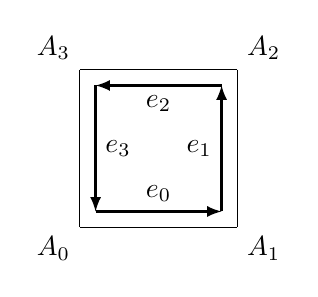
\begin{tikzpicture}
    \coordinate (A0) at (0,0);
    \coordinate (A1) at (2,0);
    \coordinate (A2) at (2,2);
    \coordinate (A3) at (0,2);
    \coordinate (B0) at (0.2,0.2);
    \coordinate (B1) at (1.8,0.2);
    \coordinate (B2) at (1.8,1.8);
    \coordinate (B3) at (0.2,1.8);
      \draw(A0)
        -- (A1) node [below right] {$A_1$};
      \draw (A1)
        -- (A2) node [above right] {$A_2$};
      \draw (A2)
        -- (A3) node [above left] {$A_3$};
      \draw (A3)
        -- (A0) node [below left] {$A_0$};
      \draw  [thick,-latex] (B0)
        -- (B1);
      \draw [thick,-latex,] (B1)
        -- (B2);
      \draw [thick,-latex,] (B2)
        -- (B3);
      \draw [thick,-latex,] (B3)
        -- (B0);
      \node [right] at (0.2, 1) {$e_3$};
      \node [above] at (1, 0.2) {$e_0$};
      \node [left] at (1.8, 1) {$e_1$};
      \node [below] at (1, 1.8) {$e_2$};
  \end{tikzpicture}
  \caption{A quadrilateral face made with four halfedges}
  \label{figure:singleFace}
\end{figure}

Every element stores two types of information: self-information and adjacency information. As shown in Table \ref{table:vhfInfo}. The adjacency information include adjacency in a face and adjacency between faces. The adjacency between faces include sibling links and boundary links. (And we will discussion more in the mesh section.) 

%Table2
\begin{table}[ht]
\centering
\begin{tabular}{| l | p{0.4\textwidth} | p{0.4\textwidth}|}

\hline
Element & Self-Information & Adjacency Information  \\
\hline
Vertex  & 1. vertex ID & 1. one outgoing halfedge   \\
& 2. vertex position & 2. on mobius connection? \\
& 3. vertex normal & \\
\hline
Halfedge & 1. edge ID & 1. start and end vertex\\
& & 2. link to parent face\\
& & 3. predecessor and successor in the parent face\\
& & 4. sibling links to adjacent face\\
& & 5. boundary links to adjacent face \\
\hline
Face    &  1. face ID & 1. one side halfedge\\
& 2. face normal &\\
\hline
\end{tabular}
\caption{Definitions and assumptions of vertex, halfedge, and face} 
\label{table:vhfInfo}
\end{table}

\subsection{Mesh}
We define a mesh as a collection of basic elements (i.e. vertex, halfedge, and face). Hashtable is implemented to represent the collection in this project, because of its constant serach time for element. We construct three hashtables for all vertices, halfedges, and faces in the mesh respectively. The keys for these hashtable are element IDs and the contents are the element pointers.

The ID of a halfedge is related with the IDs of its start vertex and end vertex. In this project, we define the ID of a halfedge as start vertex ID * maximum number of vertices in a mesh + end vertex ID. This definition will guarantee a unique ID for every halfedge when they have a different start or different end vertex from other halfedges. 

A mesh also includes the adjacency and connectivity for elements within. They can be classifed into three groups: 1) halfedge flow in an single face, 2) face connections, and 3) boundary connections.

\subsubsection{Halfedge Flow in One Face}
A face is constructed by a loop of consecutive halfedges. The start of one halfedge is the end of its previous halfedge, and the end is the start of its next halfedge. Every halfedge contains two pointers, pointing to its previous and next halfedge respectively. Every vertex in this face will also have a pointer to its outgoing halfedge.

\subsubsection{Face Connections and Sibling Links}

There are two types of face connections, the normal connection and the mobius connection, as shown in Figure \ref{figure:faceConnections}. In a typical halfedge data structure, with the assumption of double-sided surface, a pair of halfedges between two faces are defined with opposite direction. We extends this idea to represent single-sided surface by adding another type of connection, named as mobius connection. In a mobius connection, a pair of halfedges are in same direction. The vertex on a mobius connection will also be marked for the purpose of vertex traversal in the future. In the example of Figure \ref{figure:faceConnections}, on the top, $e_1$ and $e_1'$ are siblings to each other. On the bottom, $e_1$ and $e_1'$ are mobius siblings to each other. 

One thing to point out is that mobius sibling halfedges have the same element ID. Because they have the start vertex and end vertex. However, we could check for the mobius sibling pointers in order to find all halfedges in the edge traveral of a mesh.

With the extension of mobius connection, there can be three different adjacent situations for a halfedge in a mesh: 1) it is on a normal connection and has a normal sibling, 2) it is on a mobius connection and has a mobius pointer, and 3) it lies on the boundary of the surface and does not have a sibling pointer nor a mobius poniter.

%Figure2
\begin{figure}[ht]
  \centering
  %Normal Junction
  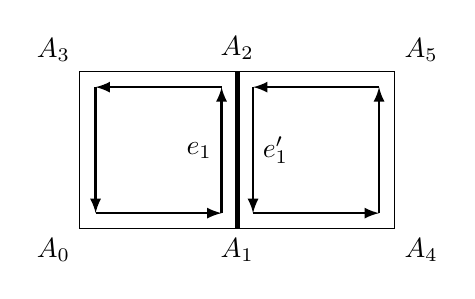
\begin{tikzpicture}
    \coordinate (A0) at (0,0);
    \coordinate (A1) at (2,0);
    \coordinate (A2) at (2,2);
    \coordinate (A3) at (0,2);
    \coordinate (A4) at (4,0);
    \coordinate (A5) at (4,2);
    \coordinate (B0) at (0.2,0.2);
    \coordinate (B1) at (1.8,0.2);
    \coordinate (B2) at (1.8,1.8);
    \coordinate (B3) at (0.2,1.8);
    \coordinate (B4) at (2.2,0.2);
    \coordinate (B5) at (3.8,0.2);
    \coordinate (B6) at (3.8,1.8);
    \coordinate (B7) at (2.2,1.8);
      \draw(A0) -- (A1) node [below] {$A_1$};
      \draw [ultra thick] (A1) -- (A2) node [above] {$A_2$};
      \draw (A2) -- (A3) node [above left] {$A_3$};
      \draw (A3) -- (A0) node [below left] {$A_0$};
      \draw (A1) -- (A4) node [below right] {$A_4$};
      \draw (A4) -- (A5) node [above right] {$A_5$};
      \draw (A5) -- (A2);
      \draw  [thick,-latex] (B0)
        -- (B1);
      \draw [thick,-latex,] (B1)
        -- (B2);
      \draw [thick,-latex,] (B2)
        -- (B3);
      \draw [thick,-latex,] (B3)
        -- (B0);
      \draw  [thick,-latex] (B4)
        -- (B5);
      \draw [thick,-latex,] (B5)
        -- (B6);
      \draw [thick,-latex,] (B6)
        -- (B7);
      \draw [thick,-latex,] (B7)
        -- (B4);
      \node [left] at (1.8, 1) {$e_1$};
      \node [right] at (2.2, 1) {$e_1'$};
  \end{tikzpicture}
  
  %Mobius Junction
  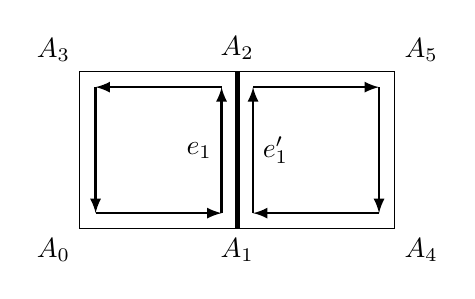
\begin{tikzpicture}
    \coordinate (A0) at (0,0);
    \coordinate (A1) at (2,0);
    \coordinate (A2) at (2,2);
    \coordinate (A3) at (0,2);
    \coordinate (A4) at (4,0);
    \coordinate (A5) at (4,2);
    \coordinate (B0) at (0.2,0.2);
    \coordinate (B1) at (1.8,0.2);
    \coordinate (B2) at (1.8,1.8);
    \coordinate (B3) at (0.2,1.8);
    \coordinate (B4) at (2.2,0.2);
    \coordinate (B5) at (3.8,0.2);
    \coordinate (B6) at (3.8,1.8);
    \coordinate (B7) at (2.2,1.8);
      \draw(A0) -- (A1) node [below] {$A_1$};
      \draw [ultra thick] (A1) -- (A2) node [above] {$A_2$};
      \draw (A2) -- (A3) node [above left] {$A_3$};
      \draw (A3) -- (A0) node [below left] {$A_0$};
      \draw (A1) -- (A4) node [below right] {$A_4$};
      \draw (A4) -- (A5) node [above right] {$A_5$};
      \draw (A5) -- (A2);
      \draw  [thick,-latex] (B0)
        -- (B1);
      \draw [thick,-latex,] (B1)
        -- (B2);
      \draw [thick,-latex,] (B2)
        -- (B3);
      \draw [thick,-latex,] (B3)
        -- (B0);
      \draw  [thick,-latex] (B5)
        -- (B4);
      \draw [thick,-latex,] (B4)
        -- (B7);
      \draw [thick,-latex,] (B7)
        -- (B6);
      \draw [thick,-latex,] (B6)
        -- (B5);
      \node [left] at (1.8, 1) {$e_1$};
      \node [right] at (2.2, 1) {$e_1'$};
  \end{tikzpicture}
  \caption{Normal connection (up) and mobius connection (down) between two faces}
  \label{figure:faceConnections}
\end{figure}

\subsubsection{Boundary and Boundary Links}

For halfedges on the boundary of a mesh, we connect them with boundary links. In a surface with no mobius connetion, the boundary halfedges follows a continous flow. We can traverse the boundary when starting at one vertex, following the natural flow on the boundary, and ending at the starting vertex. Previous boundary pointerss and next boundary pointers are created to link these halfedges. When mobius connection occurs in a mesh, however, some adjacent boundary halfedges will start or end at same vertex, which blocks the natural flow of boundary halfedges. If this happens, we build mobius boundary pointers to link these halfedges. Figure X shows an example of boundary halfedges with and without mobius connections.

<Add normal boundary links figure and mobius boundary link figures here!>

\subsubsection{Build Mesh from Elements}

As a conclusion of adjacency in a mesh, we need four steps in order to construct a mesh from basic elements.

Step 1: Create individual vertices. We create instances of vertices with their position and ID. The position of two vertices can be the same but their ID should always be unique. 

This step takes O(V) time, where V is the number of vertices in the mesh.

Step 2: Construct indivdual faces. To build an indivdual face, we create consecutive instances of halfedges, with their start and end vertices. Meanwhile, every vertex will be asigned a pointer to its outgoing halfedge when we create halfedges. For each halfedge, We then add the previous and next pointers to its previous halfedge and next halfedge respectively. 

This step takes O(E) time, where E is the number of halfedges in the mesh.

Step 3: Build sibling links. For every halfedge, we need to find if there exist a sibling or mobius sibling from other faces in this mesh. If its start vertex is same with the end of another halfedge, and its end vertex is same with the start of another halfedge, we then find a sibling. If it has the same start and end vertex with another halfedge, we then find a mobius sibling. 

In this project, with the implementation of hashtable, the ID of a halfedge is related with its start vertex ID and end vertex ID. The mobius sibling link is actually generated in step 2. When we create the halfedge, if its ID is equal to a halfedge that we created before, we know they are mobius siblings. The search of normal sibling is also in constant time because we can calculate the ID of its sibling halfedge knowing that their start and end vertex are reversed. 

This step takes O(E) time, where E is number of halfedges in the mesh.

Step 4: Build boundary links. After step 3, if a halfedge does not have a sibling or mobius sibling, it lies on the boundary of this mesh. We need to build the boundary links to these halfedges.

To do this, we need a counter to keep track of how many times we cross a mobius connection. We 1) set counter equal to zero and start from one halfedge on the boudary, 2) we go to its next halfedge if the counter is even, or its previous halfedge if the counter is odd, 3) we then go to its the sibling or moibus sibling, the counter increase by 1 if it is a mobius sibling, 4) check if the current halfedge is on boundary, if not, we repeat 2) and 3) until we reach to one, and 5) this boundary halfedge shares one vertex with our last boundary halfedge, so we can build boundary links between them, and 6) we repeat 1) to 5) to build bounary links until we reach the starting boundary halfedge in 1). From 1) to 6), one boundary loop of this mesh is built. And we move on to build other loops by repeating 1) to 6), until every boundary halfedges have boundary links to its adjacent boundaries.

This step takes O(E) time, where E is the number of halfedges in the mesh.

Now this mesh contains everything that we need to start a Catmull-Clark subdivision. It takes O(E) time from step 1 to step 4 as a summary.


\subsection{Mesh Traversals} 
The Catmull-Clark also requires two types of traversals in a mesh: 1) traversal around a face, and 2) traversal around a vertex. Traversal around a face is necessary to build face points and calculate face normals in the face. Traversal around a vertex is necessary to build vertex points and calculate vertex normals in the face.

\subsubsection{Traversal Around Face}
The traversal around a face lead to all the edges and vertices belong to this face. It starts from one side halfedge of this face, follows the halfedge flow, and ends at starting the halfedge of the traversal.
Traversals of all faces in a mesh takes O(E) time, where E is the number of faces in the mesh.

\subsubsection{Traversal Around Vertex}
The traversal around a vertex lead to all edges and faces that contains this vertex. The traversal of a vertex need to consider two issues: 1) is this vertex on a boundary, and  2) is this vertex on a mobius connection. This makes four different types of vertex traversals. See Figure \ref{figure:traversalAroundVertexNormal} - \ref{figure:traversalAroundVertexMobiusB} for examples.

In the vertex traversal without boundary and mobius issue, we start from one outgoing halfedge of this vertex. We continue to go to the next outgoing halfedge by going to the successor of its sibling until we hit the first outgoing halfedge. In the example of Figure \ref{figure:traversalAroundVertexNormal}, if start and end at halfedge $e_1$, the sequence of traversal is: $e_1$ (sibling link to) $e_1'$ (successor link to) $e_2$ (sibling link to) $e_2'$ (successor link to) $e_3$ (sibling link to) $e_3'$ (successor link to) $e_4$ (sibling link to ) $e_4'$  (successor link to)  $e_1$.

In order to address the issue of a vertex on boundary, instead of using sibling links, we use boundary links. In the example of Figure \ref{figure:traversalAroundVertexNormalB}, we have a boundary $e_4'$ to $e_2$. If start and end at halfedge $e_1$, the sequence of traversal is: $e_1$ (sibling link to) $e_1'$ (successor link to) $e_2$ (boundary link to) $e_4'$ (successor link to)  $e_1$.

To address the issue of vertex on a mobius connection, instead of using normal links, we use mobius links. At the same time, we switch between the successor and predecessor to the sibling every time we hit a mobius connection.  In the example of Figure \ref{figure:traversalAroundVertexNormal}, $e_1$ to $e_1'$ and $e_3$ to $e_3'$ have mobius siblings rather than normal sibling. If start and end at halfedge $e_1$, the sequence of traversal is: $e_1$ (mobius sibling link to) $e_1'$ (predecessor link to) $e_2$ (sibling link to) $e_2'$ (predecessor link to) $e_3$ (mobius sibling link to) $e_3'$ (successor link to) $e_4$ (sibling link to ) $e_4'$  (successor link to)  $e_1$.

If boundary and mobius connection both occur, we use a combination of the two methods above. In the example of Figure \ref{figure:traversalAroundVertexNormal}, $e_1$ to $e_1'$ and $e_3$ to $e_3'$ have mobius siblings rather than normal sibling and we have a mobius boundary connection between $e_4'$ and $e_2$. If start end end at halfedge $e_1$, the sequence of traversal is: $e_1$ (mobius sibling link to) $e_1'$ (predecessor link to) $e_2$ (mobius boundary link to ) $e_4'$  (successor link to)  $e_1$.

As a summary of the four different situations above, in a vertex traversal, we 1) start the traversal from with one outgoing halfedge of the vertex, 2) go to sibling or boundary link halfedge, 3) go to the next or previous halfedge that contains the vertex as one end, and 4) repeat 2) and 3) until we reach to the starting outgoing halfedge. This vertex traversal runs in O(E) time, where E is the total number of halfedges in the mesh.

%Figure3
\begin{figure}[ht]
  \centering
  %Normal Junction
  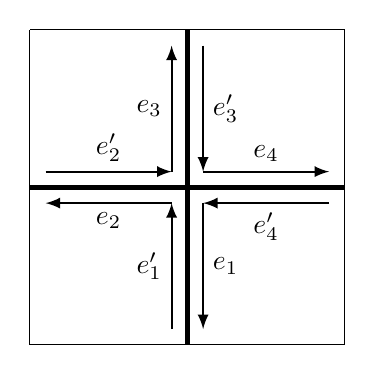
\begin{tikzpicture}
    \coordinate (A0) at (0,0);
    \coordinate (A1) at (2,0);
    \coordinate (A2) at (2,2);
    \coordinate (A3) at (0,2);
    \coordinate (A4) at (4,0);
    \coordinate (A5) at (4,2);
    \coordinate (A6) at (4,4);
    \coordinate (A7) at (2,4);
    \coordinate (A8) at (0,4);
    
    \coordinate (B0) at (0.2,0.2);
    \coordinate (B1) at (1.8,0.2);
    \coordinate (B2) at (1.8,1.8);
    \coordinate (B3) at (0.2,1.8);
    \coordinate (B4) at (2.2,0.2);
    \coordinate (B5) at (3.8,0.2);
    \coordinate (B6) at (3.8,1.8);
    \coordinate (B7) at (2.2,1.8);
    \coordinate (B8) at (0.2,2.2);
    \coordinate (B9) at (1.8,2.2);
    \coordinate (B10) at (1.8,3.8);
    \coordinate (B11) at (0.2,3.8);
    \coordinate (B12) at (2.2,2.2);
    \coordinate (B13) at (3.8,2.2);
    \coordinate (B14) at (3.8,3.8);
    \coordinate (B15) at (2.2,3.8);

     \draw (A0) -- (A1);
     \draw [ultra thick](A1) -- (A2);
     \draw  [ultra thick](A2) -- (A3);
     \draw (A3) -- (A0);
     \draw (A1) -- (A4);
     \draw (A4) -- (A5);
     \draw [ultra thick](A5) -- (A2);
     \draw (A3) -- (A8);
     \draw (A8) -- (A7);
     \draw (A7) -- (A6);
     \draw (A6) -- (A5);
     \draw [ultra thick] (A7) -- (A2);

     \draw [thick,-latex,] (B1) -- (B2);
     \draw [thick,-latex,] (B2) -- (B3);
     \draw [thick,-latex,] (B6) -- (B7);
     \draw [thick,-latex,] (B7) -- (B4);
     \draw [thick,-latex,] (B8) -- (B9);
     \draw  [thick,-latex] (B9) -- (B10);
     \draw [thick,-latex,] (B15) -- (B12);
     \draw [thick,-latex,] (B12) -- (B13);
     \node [left] at (1.8, 1) {$e_1'$};
     \node [right] at (2.2, 1) {$e_1$};
     \node [left] at (1.8, 3) {$e_3$};
     \node [right] at (2.2, 3) {$e_3'$};
     \node [below] at (1, 1.8) {$e_2$};
     \node [above] at (1, 2.2) {$e_2'$};
     \node [below] at (3, 1.8) {$e_4'$};
     \node [above] at (3, 2.2) {$e_4$};
  \end{tikzpicture}
  \caption{Vertex traversal without boundary and without moibus connection}
  \label{figure:traversalAroundVertexNormal}
\end{figure}
%Figure 4
\begin{figure}[ht]
  \centering
  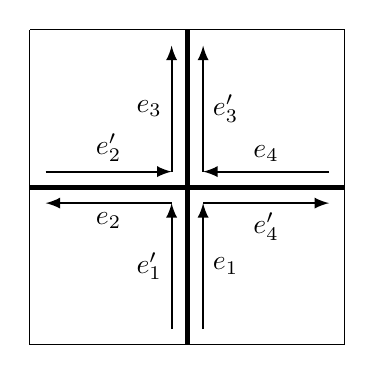
\begin{tikzpicture}
    \coordinate (A0) at (0,0);
    \coordinate (A1) at (2,0);
    \coordinate (A2) at (2,2);
    \coordinate (A3) at (0,2);
    \coordinate (A4) at (4,0);
    \coordinate (A5) at (4,2);
    \coordinate (A6) at (4,4);
    \coordinate (A7) at (2,4);
    \coordinate (A8) at (0,4);
    
    \coordinate (B0) at (0.2,0.2);
    \coordinate (B1) at (1.8,0.2);
    \coordinate (B2) at (1.8,1.8);
    \coordinate (B3) at (0.2,1.8);
    \coordinate (B4) at (2.2,0.2);
    \coordinate (B5) at (3.8,0.2);
    \coordinate (B6) at (3.8,1.8);
    \coordinate (B7) at (2.2,1.8);
    \coordinate (B8) at (0.2,2.2);
    \coordinate (B9) at (1.8,2.2);
    \coordinate (B10) at (1.8,3.8);
    \coordinate (B11) at (0.2,3.8);
    \coordinate (B12) at (2.2,2.2);
    \coordinate (B13) at (3.8,2.2);
    \coordinate (B14) at (3.8,3.8);
    \coordinate (B15) at (2.2,3.8);

     \draw (A0) -- (A1);
     \draw [ultra thick](A1) -- (A2);
     \draw  [ultra thick](A2) -- (A3);
     \draw (A3) -- (A0);
     \draw (A1) -- (A4);
     \draw (A4) -- (A5);
     \draw [ultra thick](A5) -- (A2);
     \draw (A3) -- (A8);
     \draw (A8) -- (A7);
     \draw (A7) -- (A6);
     \draw (A6) -- (A5);
     \draw [ultra thick] (A7) -- (A2);

     \draw [thick,-latex,] (B1) -- (B2);
     \draw [thick,-latex,] (B2) -- (B3);
     \draw [thick,-latex,] (B7) -- (B6);
     \draw [thick,-latex,] (B4) -- (B7);
     \draw [thick,-latex,] (B8) -- (B9);
     \draw [thick,-latex] (B9) -- (B10);
     \draw [thick,-latex,] (B13) -- (B12);
     \draw [thick,-latex,] (B12) -- (B15);
     \node [left] at (1.8, 1) {$e_1'$};
     \node [right] at (2.2, 1) {$e_1$};
     \node [left] at (1.8, 3) {$e_3$};
     \node [right] at (2.2, 3) {$e_3'$};
     \node [below] at (1, 1.8) {$e_2$};
     \node [above] at (1, 2.2) {$e_2'$};
     \node [below] at (3, 1.8) {$e_4'$};
     \node [above] at (3, 2.2) {$e_4$};  \end{tikzpicture}
  \caption{Vertex traversal without boundary and with moibus connection}
  \label{figure:traversalAroundVertexMobius}
\end{figure}
%Figure4
\begin{figure}[ht]
  \centering
  %Normal Junction
  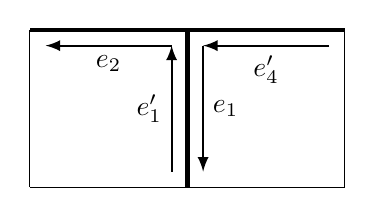
\begin{tikzpicture}
    \coordinate (A0) at (0,0);
    \coordinate (A1) at (2,0);
    \coordinate (A2) at (2,2);
    \coordinate (A3) at (0,2);
    \coordinate (A4) at (4,0);
    \coordinate (A5) at (4,2);
    
    \coordinate (B0) at (0.2,0.2);
    \coordinate (B1) at (1.8,0.2);
    \coordinate (B2) at (1.8,1.8);
    \coordinate (B3) at (0.2,1.8);
    \coordinate (B4) at (2.2,0.2);
    \coordinate (B5) at (3.8,0.2);
    \coordinate (B6) at (3.8,1.8);
    \coordinate (B7) at (2.2,1.8);

     \draw (A0) -- (A1);
     \draw [ultra thick](A1) -- (A2);
     \draw  [ultra thick](A2) -- (A3);
     \draw (A3) -- (A0);
     \draw (A1) -- (A4);
     \draw (A4) -- (A5);
     \draw [ultra thick](A5) -- (A2);

     \draw [thick,-latex,] (B1) -- (B2);
     \draw [thick,-latex,] (B2) -- (B3);
     \draw [thick,-latex,] (B6) -- (B7);
     \draw [thick,-latex,] (B7) -- (B4);
     
     \node [left] at (1.8, 1) {$e_1'$};
     \node [right] at (2.2, 1) {$e_1$};
     \node [below] at (1, 1.8) {$e_2$};
     \node [below] at (3, 1.8) {$e_4'$};
  \end{tikzpicture}
  \caption{Vertex traversal withboundary and without moibus connection}
  \label{figure:traversalAroundVertexNormalB}
\end{figure}

%Figure5
\begin{figure}[ht]
  \centering
  %Normal Junction
  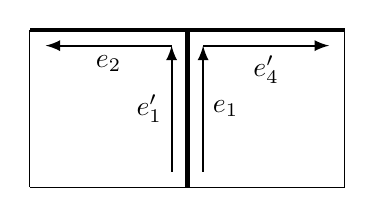
\begin{tikzpicture}
    \coordinate (A0) at (0,0);
    \coordinate (A1) at (2,0);
    \coordinate (A2) at (2,2);
    \coordinate (A3) at (0,2);
    \coordinate (A4) at (4,0);
    \coordinate (A5) at (4,2);
    
    \coordinate (B0) at (0.2,0.2);
    \coordinate (B1) at (1.8,0.2);
    \coordinate (B2) at (1.8,1.8);
    \coordinate (B3) at (0.2,1.8);
    \coordinate (B4) at (2.2,0.2);
    \coordinate (B5) at (3.8,0.2);
    \coordinate (B6) at (3.8,1.8);
    \coordinate (B7) at (2.2,1.8);

     \draw (A0) -- (A1);
     \draw [ultra thick](A1) -- (A2);
     \draw  [ultra thick](A2) -- (A3);
     \draw (A3) -- (A0);
     \draw (A1) -- (A4);
     \draw (A4) -- (A5);
     \draw [ultra thick](A5) -- (A2);

     \draw [thick,-latex,] (B1) -- (B2);
     \draw [thick,-latex,] (B2) -- (B3);
     \draw [thick,-latex,] (B7) -- (B6);
     \draw [thick,-latex,] (B4) -- (B7);
     
     \node [left] at (1.8, 1) {$e_1'$};
     \node [right] at (2.2, 1) {$e_1$};
     \node [below] at (1, 1.8) {$e_2$};
     \node [below] at (3, 1.8) {$e_4'$};

  \end{tikzpicture}
  \caption{Vertex traversal with boundary and with moibus connection}
  \label{figure:traversalAroundVertexMobiusB}
\end{figure}

\subsection{Mesh Operations}
Building from basic elements is not the only way to construct a mesh. A new mesh can also be made by copy a

\subsubsection{Instantiation and Rotation}
\subsubsection{Build by Merging Meshes}

\section{Catumll-Clark Subdivision} \label{sec:ccsd}

\subsection{General Approach of Catmull-Clark Subdivision}

\subsubsection{Compute Vertex Positions of New Mesh}

\subsubsection{Make Connections of New Mesh}

\subsection{Sharp Crease and Boundary Feature}

\subsection{Mobius Connection}

\section{Offset Surface} \label{sec:offset}

\subsection{Compute Vertex Normals}

\subsection{Positive and Negative Offsets}

\subsection{Mobius Connection Issue}

\section{Input and Output}

\section{Test Cases and Discussions}

\section{Future Researches}


\end{document}